%-------------------------------------------------------------------------------------------------
%         TEXT
%-------------------------------------------------------------------------------------------------
%-------------- Introduction
\newcommand{\intro}{

\begin{alertblock}{The Method of Geometric Optics}
\setbeamercolor{item}{fg=\alertblockitem}
\captionsetup[figure]{labelfont={color=\alertblockcaption}}
\begin{itemize}
\item The idea of the method is to use \textbf{straight lines (rays)} to model waves. 
\\
\begin{centering}
\begin{figure}
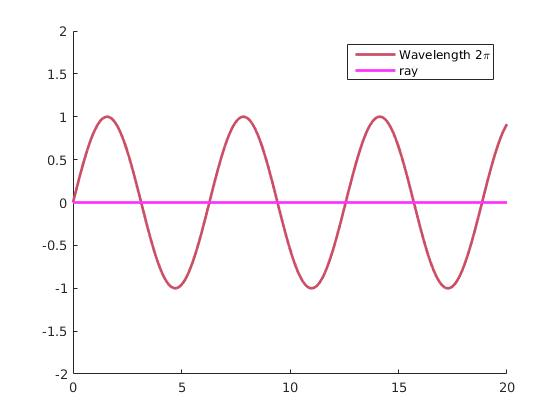
\includegraphics[width=0.85\linewidth]{WaveRay.jpg}
\end{figure} 
\end{centering}
\item \textbf{Rays} are mapped around an environment from source to visualise the path of the waves. An example is given in Figure \ref{fig::rayfield}. 
\\
\begin{figure}
\begin{centering}
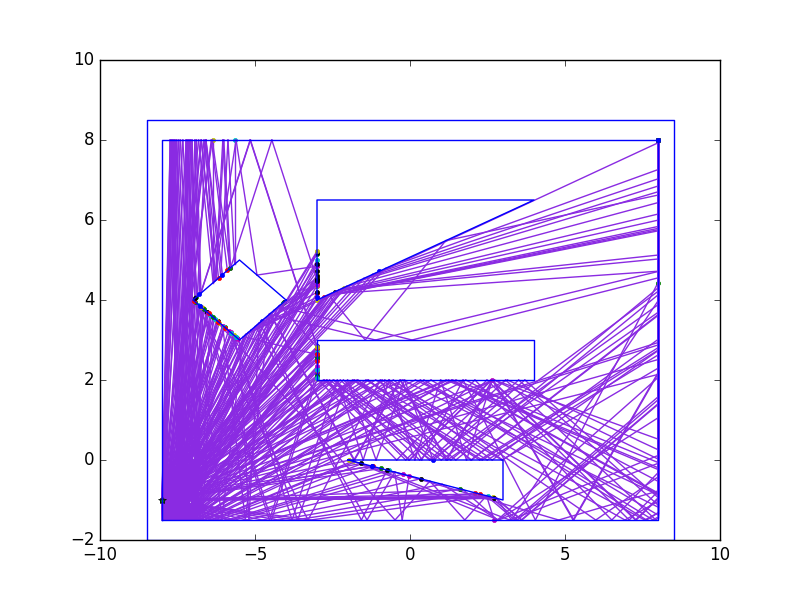
\includegraphics[width=0.85\linewidth]{Rayfield.png}
\caption{\textcolor{black}{Rays propagating from a source and reflecting within an environment. \label{fig::rayfield} }}
\end{centering}
\end{figure}
\item \textbf{Field of rays} is then observed to give an overview of the results in the environment. 
\item Calculations are then made \textbf{along the ray} and hence \textbf{over the ray field} to determine information about the \textbf{properties wave}. 
\item \textbf{Ray-tracing} requires the wave-length to be small relative to the dimensions of the environment.
\end{itemize}
\end{alertblock}

}




%-------------- First Block
\newcommand{\firstblock}{•}






%-------------- Second Block
\newcommand{\secondblock}{•}






%-------------- Third Block
\newcommand{\thirdblock}{•}




%-------------- conclusion
\newcommand{\conclusion}{•}